\section{Experiments}
\label{sec:experiment}
We evaluate our method against other state-of-the-art 3D Language Gaussian Splatting methods on open vocabulary segmentation and localization tasks, as well as compare their computational efficiency metrics. Additionally, we analyze how our method scales across different feature dimensions, examining the trade-offs between dimensionality, computational requirements, and segmentation quality.

\begin{figure}[t]
    \centering
    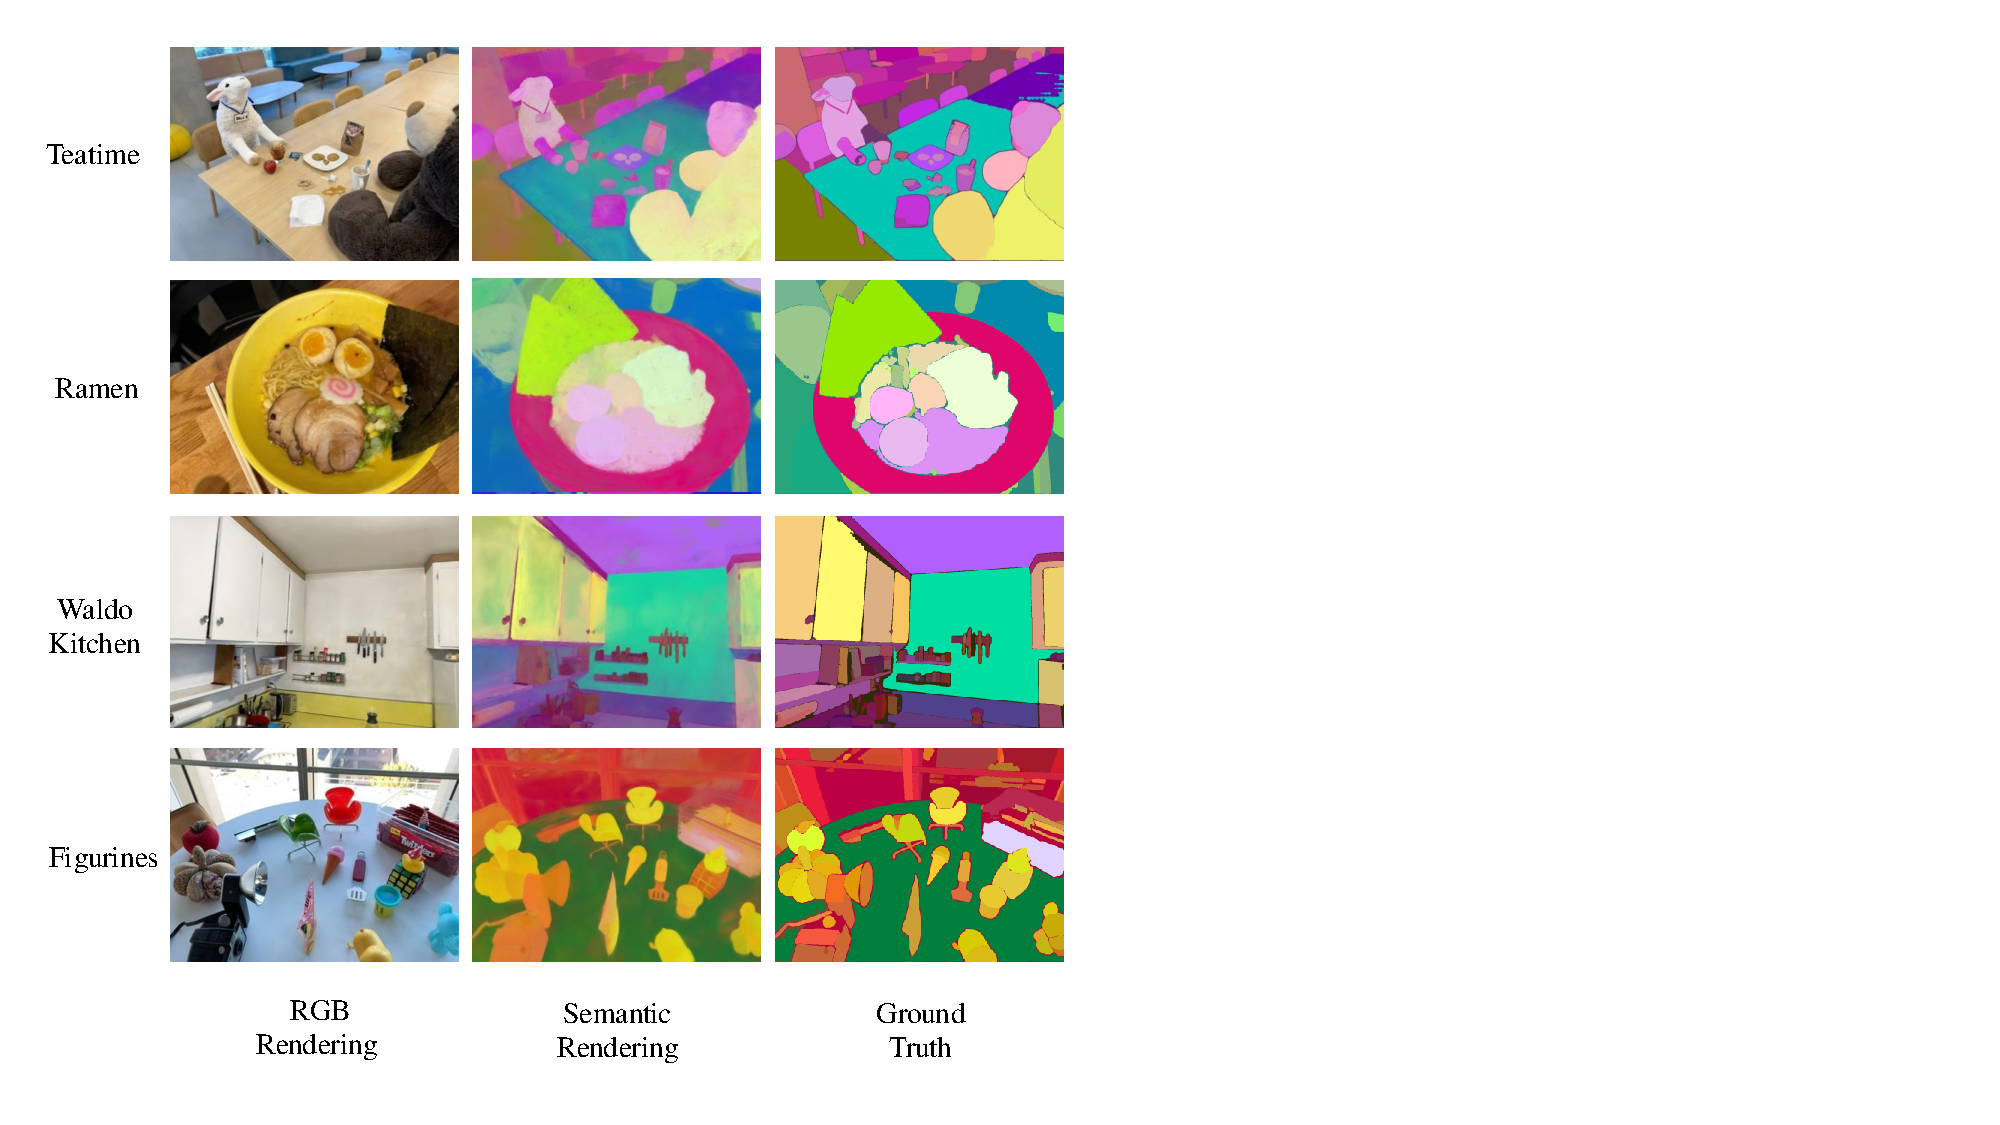
\includegraphics[width=0.88\textwidth]{figures/lerf_vis2.pdf}
    \caption{PCA visualization of semantic features on LERF Dataset. (a) Original RGB rendering. (b) PCA visualization of our rendered semantic feature maps. (c) Initial semantic feature maps extracted using CLIP from SAM segmentations. }
    \label{fig:lerf-vis}
\end{figure}

\subsection{Dataset} To assess the effectiveness of our method, we evaluate it on two widely used datasets: LERF~\cite{kerr2023lerf} and 3D-OVS~\cite{liu2023weakly}. The LERF dataset features everyday indoor scenes with diverse objects and we perform quantitative evaluations on the commonly used scenes Ramen, Figurines, Teatime, and Waldo Kitchen according to the LERF evaluation protocol~\cite{kerr2023lerf}. For these scenes, we evaluate both open-vocabulary segmentation (mIoU) and localization accuracy. The 3D-OVS dataset contains long-tail objects in diverse backgrounds, and we evaluate segmentation performance on five scenes: sofa, lawn, bed, room, and bench. For evaluation, we utilize the annotations provided by~\cite{qin2024langsplat} for both datasets.

\subsection{Implementation Details}
Our implementation of Occam's LGS is built on gsplat~\cite{ye2024gsplatopensourcelibrarygaussian}, a CUDA-accelerated Gaussian rendering library that supports high-dimensional feature rendering. For each scene, we train a 3D Gaussian Splatt for 30,000 iterations using the common Gaussian Splatting~\cite{kerbl3Dgaussians} parameters, resulting in an average number of 2,500,000 Gaussians for RGB representation across scenes. To ensure a fair comparison, we follow the 2D language feature map generation method from~\cite{qin2024langsplat}. For language feature extraction and segmentation, our pipeline integrates OpenCLIP ViT-B/16~\cite{Radford2021LearningTV} and SAM ViT-H~\cite{kirillov2023segment}. To capture semantic information hierarchically, we generate 2D feature maps at three levels:  whole, part, and subpart, where each level represents distinct semantic granularity. Following the feature extraction, we use our method to uplift the 2D language features to 3D scenes using training views only, and evaluate the results on separate testing views, withheld during training of the semantic representation. All experiments and runtime measurements are conducted on a single NVIDIA A6000 GPU. 

For the LERF dataset, we follow the LERF~\cite{kerr2023lerf} evaluation protocol, computing relevancy scores between query text and rendered 2D feature maps with a mask threshold of 0.5. For 3D-OVS, we first normalize the rendered feature maps to ensure comparable relevancy scores across classes, then apply dynamic thresholding detailed in the supplementary material. During thresholding, we reject spurious masks with areas smaller than 0.005\% or larger than 0.90\% of the image and set an object stability threshold of 0.4.

\subsection{Open Vocabulary Semantic Segmentation}
Given a 3D scene and a language query describing an object or region of interest, the task of open vocabulary semantic segmentation is to identify and generate masks for all relevant regions that match a query description. We evaluate our approach against existing methods on two datasets: LERF and 3D-OVS, with quantitative results shown in Tables \ref{tab:lerf-mIoU} and \ref{tab:3dovs-mIoU} respectively and qualitative results shown in Figure \ref{fig:lerf-vis} and \ref{fig:comparison}. On the LERF dataset, under identical experimental settings as LangSplat, our approach demonstrates a substantial improvement of 9.9\% mIoU. Notably, our method shows advantages, especially in complex scenes with sparse view coverage. An example of this is Waldo Kitchen, where the camera captures an entire room rather than focusing on a specific area that is fully surrounded by camera views. 

On 3D-OVS, our method achieves state-of-the-art results, with an improvement of $1.6\%$ mIoU over the current SOTA LangSplat~\cite{qin2024langsplat}. Performance gains of 3D-OVS are less pronounced compared to LERF~\cite{kerr2023lerf}, likely since this dataset contains simpler scenes, focused on a single region with good view coverage and fewer objects, where existing methods have already saturated in performance.

\begin{table}[t]
    \centering
    \footnotesize
    \begin{tabular}{lccccc}
        \toprule
        \textbf{Method}& 
        \hspace{-2pt}\textbf{Ramen}\hspace{-2pt} & \hspace{-2pt}\textbf{Figurines}\hspace{-2pt} & \hspace{-2pt}\textbf{Teatime}\hspace{-2pt} & \hspace{-2pt}\makecell{\textbf{Waldo}\\\textbf{Kitchen}}\hspace{-2pt} & \hspace{-2pt}\textbf{Overall}\hspace{-2pt} \\
        \midrule
        LSeg & 7.0 & 7.6 & 21.7 & 29.9 & 16.6 \\
        LERF & 28.2 & 38.6 & 45.0 & 37.9 & 37.4 \\
        GS-Grouping & 45.5 & \underline{60.9} & 40.0 & 38.7 & 46.3 \\
        Feature-3DGS & 43.7 & 58.8 & 40.5 & 39.6 & 45.7 \\
        LEGaussians & 46.0 & 60.3 & 40.8 & 39.4 & 46.9 \\
        GOI & $\mathbf{52.6}$ & $\mathbf{63.7}$ & 44.5 & 41.4 & 50.6 \\
        LangSplat & $\underline{51.2}$ & 44.7 & $\underline{65.1}$ & $\underline{44.5}$ & $\underline{51.4}$ \\
        %3DVLGS & $\mathbf{61.4}$ & $\mathbf{73.5}$ & 58.1 & $\underline{54.8}$ & $\mathbf{62.0}$ \\
        Ours & 51.0 & 58.6 & $\mathbf{70.2}$ & $\mathbf{65.3}$ & $\mathbf{61.3}$ \\
        \bottomrule
    \end{tabular}
    \caption{Comparison of average IoU on LERF Dataset.}
    \label{tab:lerf-mIoU}
\end{table}
\begin{table}[t]
    \centering
    \footnotesize
    \begin{tabular}{lcccccc}
        \toprule
        \hspace{-2pt}\textbf{Method}\hspace{-2pt} &
        \hspace{-2pt}\textbf{Bed}\hspace{-2pt} &
        \hspace{-2pt}\textbf{Bench}\hspace{-2pt} &
        \hspace{-2pt}\textbf{Room}\hspace{-2pt} &
        \hspace{-2pt}\textbf{Sofa}\hspace{-2pt} &
        \hspace{-2pt}\textbf{Lawn}\hspace{-2pt} &
        \hspace{-2pt}\textbf{Overall}\hspace{-2pt}\\
        \midrule
        \hspace{-2pt}LSeg & 56.0 & 6.0 & 19.2 & 4.5 & 17.5 & 20.6\\
        \hspace{-2pt}LERF & 73.5 & 53.2 & 46.6 & 27 & 73.7 & 54.8\\
        \hspace{-2pt}GS-Grouping & 83.0 & 91.5 & 85.9 & 87.3 & 90.6 & 87.7\\
        \hspace{-2pt}Feature-3DGS\hspace{-3pt} & 83.5 & 90.7 & 84.7 & 86.9 & 93.4 & 87.8\\
        \hspace{-2pt}LEGaussians & 84.9 & 91.1 & 86.0 & 87.8 & 92.5 & 88.5\\
        \hspace{-2pt}GOI & 89.4 & 92.8 & 91.3 & 85.6 & 94.1 & 90.6\\
        \hspace{-2pt}LangSplat & $\underline{92.5}$ & $\underline{94.2}$ & $\underline{94.1}*$ & $\mathbf{90.0}$ & $\underline{96.1}$ & $\underline{93.4}$\\
        %3DVLGS & 96.8 & 97.3 & 97.7 & 95.5 & 97.9 & 97.1\\
        Ours & $\mathbf{96.8}$ & $\mathbf{95.8}$ & $\mathbf{96.5}*$ & $\underline{88.8}$ & $\mathbf{97.0}$ & $\mathbf{95.0}$\\
        \bottomrule
    \end{tabular}
    \caption{Comparison of average IoU on 3D-OVS Datasets. The utilized image resolution is 1440 $\times$ 1080. Methods with * are evaluated on testing-data that has an annotation error in the 3D-OVS testset corrected.}
    \label{tab:3dovs-mIoU}
\end{table}

\begin{figure}[h]
    \centering
    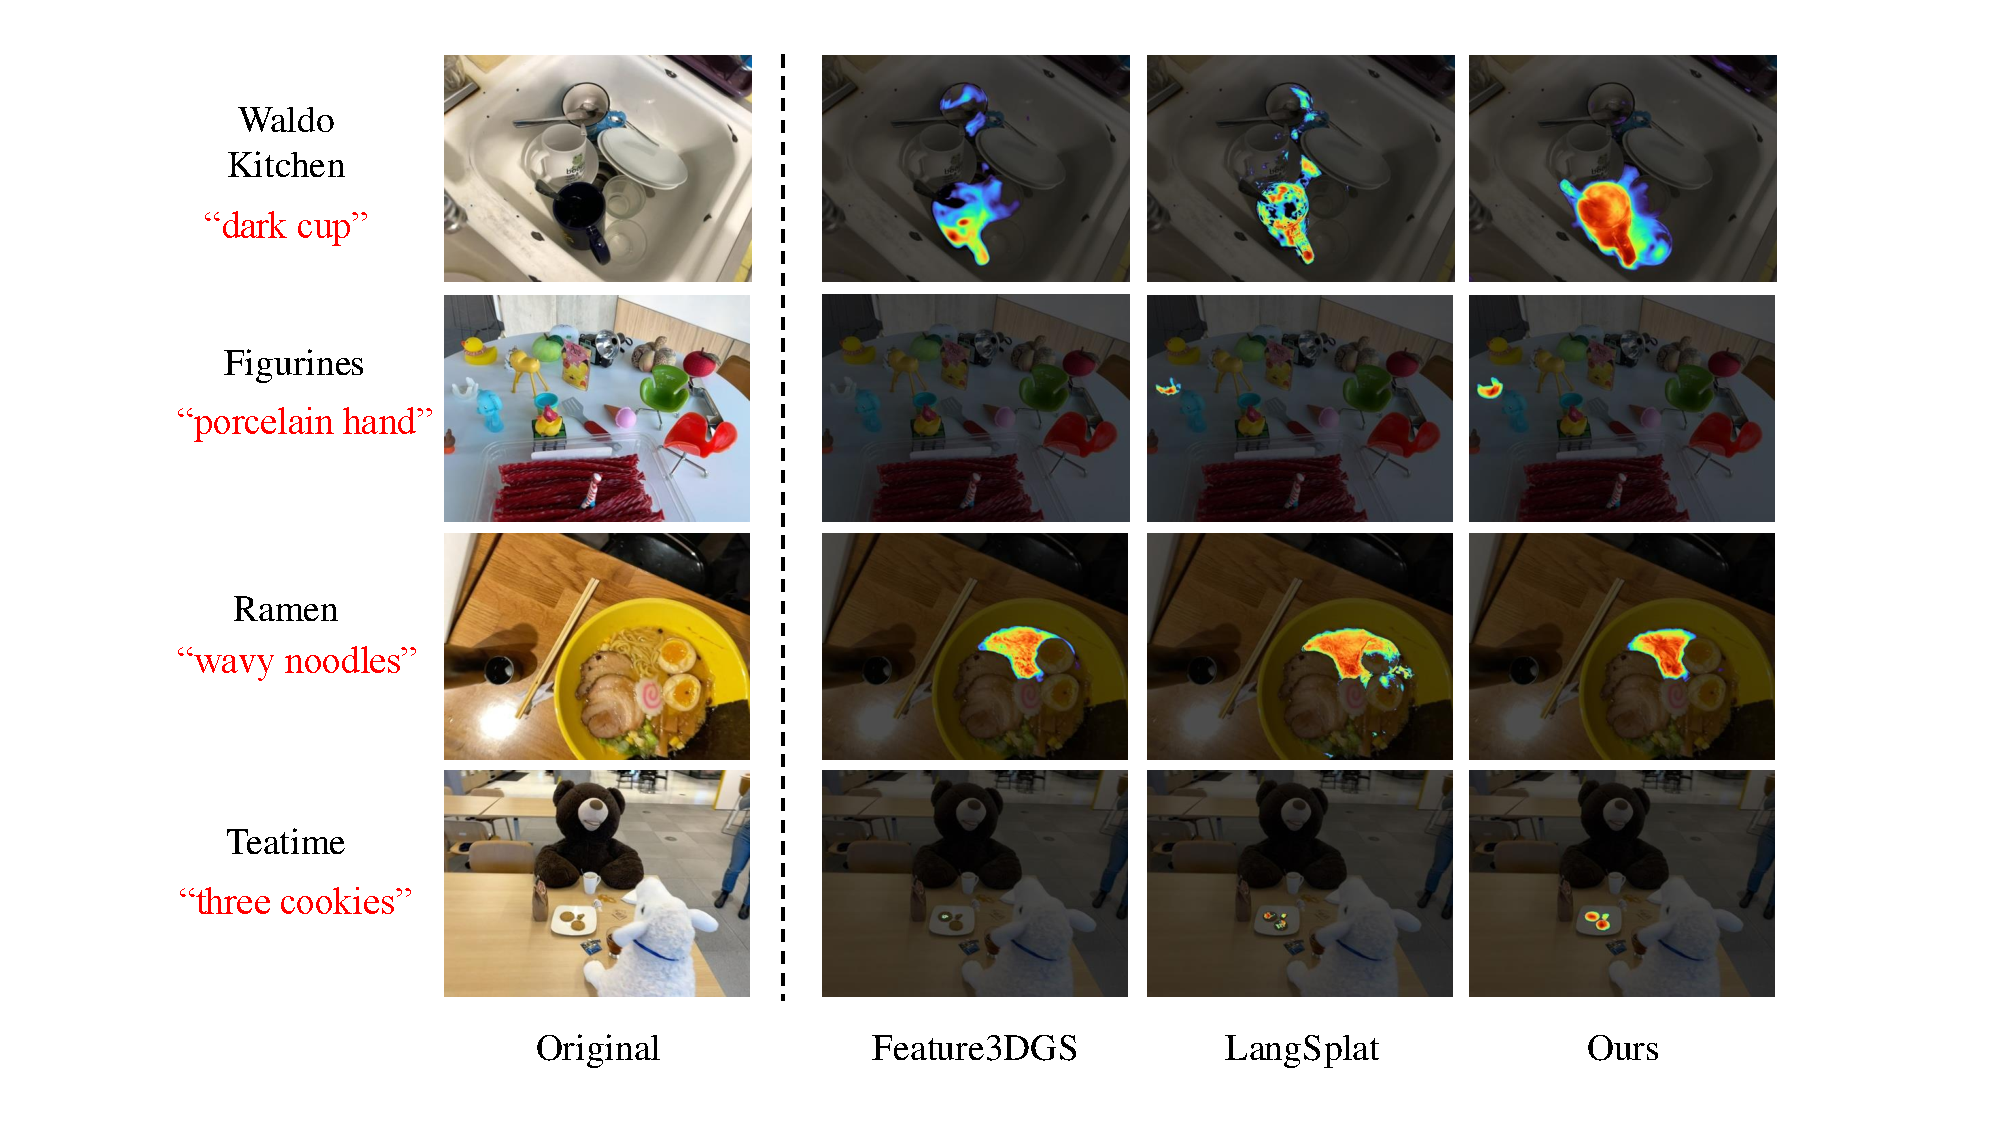
\includegraphics[trim={3cm 1cm 1cm 1cm}, clip, width=0.52\textwidth]{figures/comparison.pdf}
    \caption{Qualitative comparison of relevancy score visualization. }
    \label{fig:comparison}
\end{figure}

\subsection{Localization}
We further evaluate on the language-guided localization task, where, given a language query, the pixel with the highest relevancy score is selected, following~\cite{kerr2023lerf}. Benchmarking against existing methods, our approach achieves competitive localization accuracy, as shown by Table \ref{tab:lerf-loc-acc}.

Adding feature compression as in existing methods, increases localization accuracy of our approach to 84.1. This is due to the metric only measuring the closest matching pixel, while ignoring the feature distribution and object shape, making it prone to noise. We provide detailed experiments in this setting in the supplementary material.

\begin{table}[t]
    \centering
    \footnotesize
    \begin{tabular}{lccccc}
    \toprule
        \textbf{Method}& 
        \hspace{-2pt}\textbf{Ramen}\hspace{-2pt} & \hspace{-2pt}\textbf{Figurines}\hspace{-2pt} & \hspace{-2pt}\textbf{Teatime}\hspace{-2pt} & \hspace{-2pt}\makecell{\textbf{Waldo}\\\textbf{Kitchen}}\hspace{-2pt} & \hspace{-2pt}\textbf{Overall}\hspace{-2pt} \\
        \midrule
        LSeg & 14.1 & 8.9 & 33.9 & 27.3 & 21.1 \\
        LERF & 62.0 & 75.0 & 84.8 & 72.7 & 73.6 \\
        GS-Grouping & 68.6 & 75.0 & 74.3 & 88.2 & 76.5 \\
        Feature-3DGS & 69.8 & 77.2 & 73.4 & 87.6 & 77.0 \\
        LEGaussians & 67.5 & 75.6 & 75.2 & 90.3 & 77.2 \\
        GOI & 75.5 & $\mathbf{88.6}$ & 82.9 & $\underline{90.4}$ & $\mathbf{84.4}$ \\
        LangSplat & $\underline{73.2}$ & $\underline{80.4}$ & $\underline{88.1}$ & $\mathbf{95.5}$ & $\underline{84.3}$ \\
        %3DVLGS & 92.5 & 95.8 & 97.1 & 98.6 & 96.0 \\
        %FMGS & 90.0 & 89.7 & 93.8 & 92.6 & 91.5 \\
        Ours & $\mathbf{74.7}$ & $\underline{80.4}$ & $\mathbf{93.2}$ & 81.8 & 82.5 \\
        \bottomrule
        \end{tabular}
        \caption{Comparison of localization accuracy on LERF Datasets.}
        \label{tab:lerf-loc-acc}
\end{table}

\subsection{Robustness to Feature Dimension Variations}
\label{sec:featdim}
In the following, we demonstrate the advantages of different feature dimensions that Occam's LGS enables and assess the respective scalability and performance. For these experiments, we 1) used an autoencoder to compress the CLIP features, 2) uplifted them to 3D using our method, 3) rendered the compressed features, and 4) decompressed features to 512D using the autoencoder. Table~\ref{tab:lerf-featdim-mIoU} shows the IoU across different feature dimensions on LERF datasets. Notably, segmentation performance improves to 64.5~\%mIoU with 64D features, outperforming the LangSplat~\cite{qin2024langsplat} baseline by $13.1\%$~mIoU. This confirms that feature compression filters noise by limiting the feature space to objects present in the 3d scene, at the cost of limited scene editing capability. Since our method supports arbitrary feature dimensions, selecting this operating point is straightforward and can be used depending on the task at hand.

\begin{table}[t]
    \centering
    \footnotesize
    \begin{tabular}{lccccc}
        \toprule
        \textbf{Dimensions}& 
        \hspace{-2pt}\textbf{Ramen}\hspace{-2pt} & \hspace{-2pt}\textbf{Figurines}\hspace{-2pt} & \hspace{-2pt}\textbf{Teatime}\hspace{-2pt} & \hspace{-2pt}\makecell{\textbf{Waldo}\\\textbf{Kitchen}}\hspace{-2pt} & \hspace{-2pt}\textbf{Overall}\hspace{-2pt} \\
        \midrule
        16-D & 48.4 & 57.7 & 75.9 & 59.9 & 60.5 \\
        32-D & \textbf{53.6} & 61.8 & 78.6 & 62.6 & 64.1 \\
        64-D & 51.7 & \textbf{63.4} & \textbf{79.0} & 63.7 & \textbf{64.5} \\
        128-D & 52.1 & 62.4 & 74.3 & 62.6 & 62.9 \\
        256-D & 53.0 & 62.6 & 74.3 & 61.1 & 62.7 \\
        512-D & 51.0 & 58.6 & 70.2 & \textbf{65.3} & 61.3 \\
        \bottomrule
    \end{tabular}
    \caption{Average mIoU with varying feature dimensions on LERF scenes.}
    \label{tab:lerf-featdim-mIoU}
\end{table}

\subsection{Computational Efficiency}
We evaluate the computational efficiency of our method against existing approaches in Figure~\ref{fig:teaser} measuring their semantic Gaussian training times. Similar to ours, LangSplat and GOI both allow the integration of pre-trained 3D Gaussian models, while 3DVLM requires joint uplifting and reconstruction. %, and we trained GOI using identical feature maps as LangSplat at whole object, part, and subpart granularities. For these existing methods, we report their semantic feature training times.
LangSplat, GOI, and 3DVLM take 67, 60, and 65 minutes to uplift three levels of features respectively~\cite{peng20243dvisionlanguagegaussiansplatting}. With our approach, language features can be uplifted in 16.4 seconds without setup, and 31.9 seconds with setup (checkpoint loading and saving).
%In contrast, 3DVLM cannot utilize pre-trained Gaussians and thus, the reported time reflects their complete joint training of both reconstruction and semantics, which takes 65 minutes~\cite{peng20243dvisionlanguagegaussiansplatting}.
Overall, our method, achieves feature uplifting two orders of magnitude faster than existing methods, while delivering superior performance across test datasets and avoiding feature compression.

We assess our method's scalability through a thorough analysis of runtime, storage requirements, rendering speed, and GPU memory to uplift one feature level across four scenes of varying complexity. Additionally, we evaluate scaling across different feature dimensions, providing insights into the range of practical deployment scenarios.

The results depicted in Figure~\ref{fig:comp_efficiency}(d) demonstrate that our method scales well and maintains high computational efficiency even with large scenes containing up to 4 Million Gaussians, indicating its practical scalability across varying scene complexities. The memory requirement, shown by Figure~\ref{fig:comp_efficiency}(a) stays below 14GB for 512D CLIP features, which is met by most modern GPUs.  A key advantage of our method is its flexibility to support features of any dimension, enabling the selection of the optimal feature size for specific applications. From Figure~\ref{fig:comp_efficiency}(c), we observe that rendering speed decreases as feature dimension increases, presenting a clear trade-off between feature expressiveness and computational performance. Storage requirements similarly scale with feature dimensionality, shown by Figure~\ref{fig:comp_efficiency}(b). These findings highlight the adaptability of our approach, enabling users to balance quality, memory usage, and rendering speed based on their available resources and application requirements.


% \begin{figure*}[t]
%     \centering
%     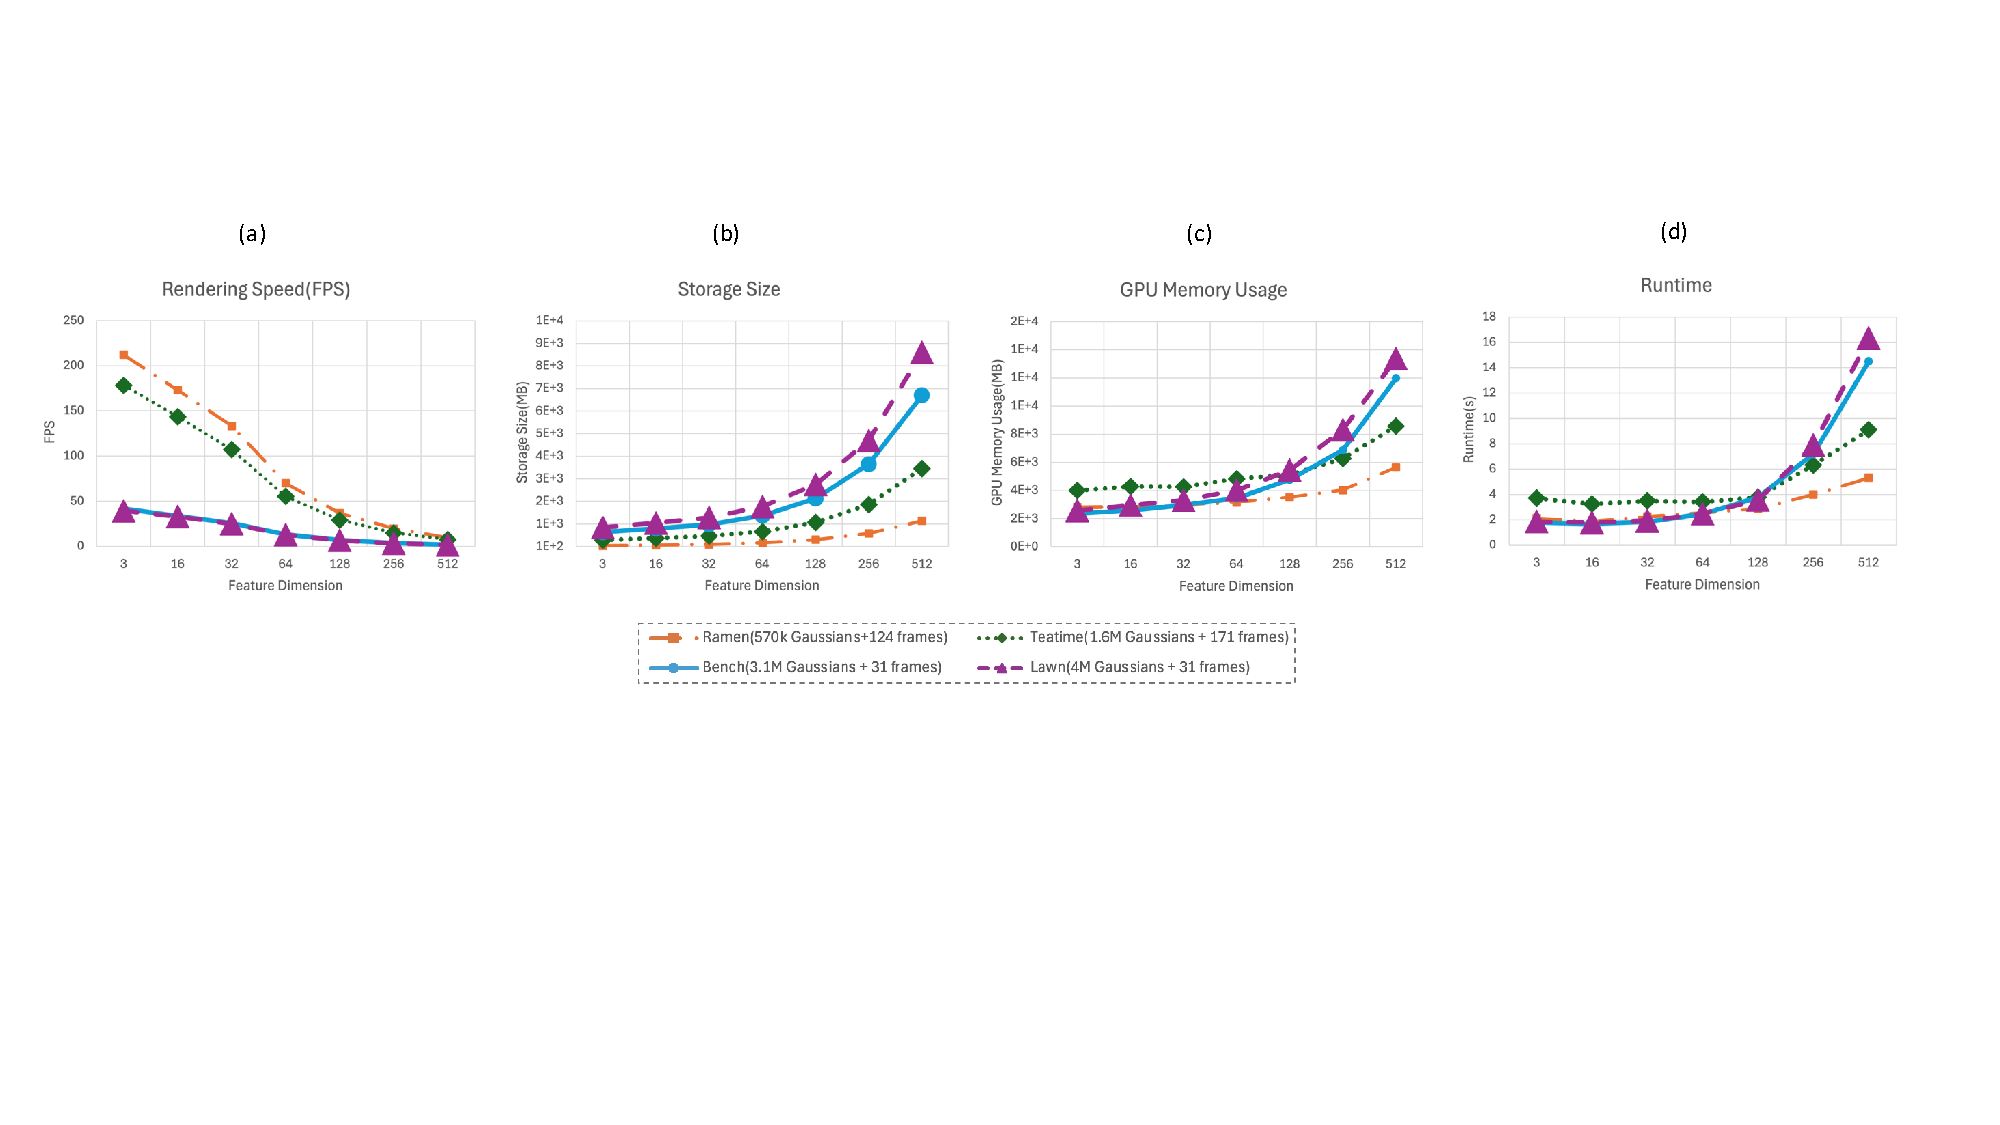
\includegraphics[width=1\textwidth, trim={20 210 20 100}, clip]{figures/computational_efficiency.pdf}
%     \caption{Comprehensive analysis of computational efficiency metrics across different feature dimensions, showing rendering speed (FPS), storage size, GPU memory usage, and runtime performance as Gaussian size and frame numbers vary.}
%     \label{fig:comp_efficiency}
% \end{figure*}


\begin{figure}[t]
    \centering
    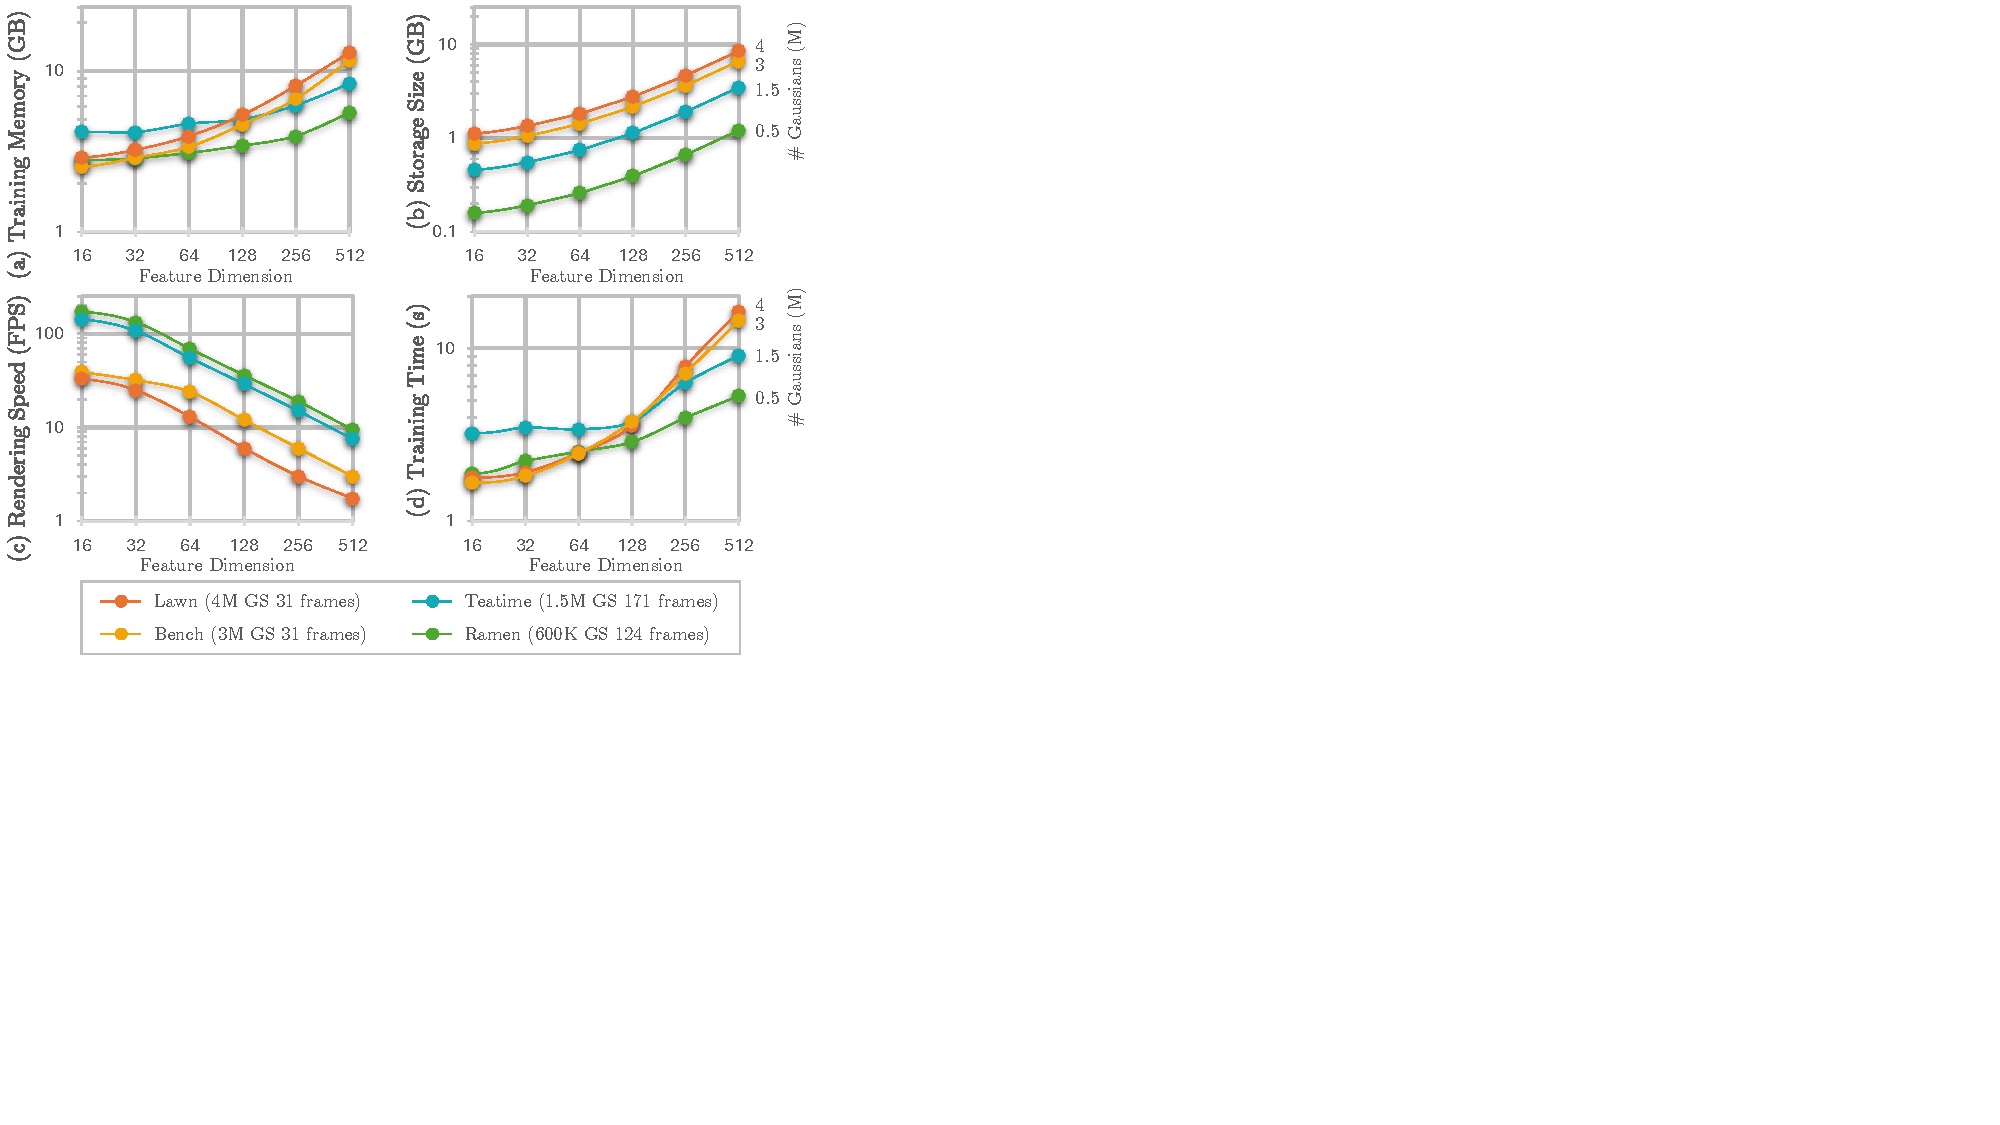
\includegraphics[width=1\textwidth, trim={0 225 150 0}, clip]{figures/efficiency_iccv.pdf}
    \caption{Comprehensive analysis of computational efficiency metrics across different feature dimensions, showing rendering speed (FPS), storage size, GPU memory usage, and runtime performance as Gaussian size and frame numbers vary.}
    \label{fig:comp_efficiency}
\end{figure}


\subsection{Ablation Study}

\begin{table}[t]
   \centering
   \footnotesize
   \begin{tabular}{lc c c c c}
       \toprule
        \textbf{Method} & \hspace{-2pt}\textbf{Ramen}\hspace{-2pt} & \hspace{-2pt}\textbf{Figurines}\hspace{-2pt} & \hspace{-2pt}\textbf{Teatime}\hspace{-2pt} & \hspace{-2pt}\makecell{\textbf{Waldo}\\\textbf{Kitchen}}\hspace{-2pt} & \hspace{-2pt}\textbf{Overall}\hspace{-2pt} \\
        \midrule
        Ours & 51.0 & 58.6 & 70.2 & 65.3 & 61.3 \\
        (w/o) wtd. agg & 45.3 & 56.7 & 70.0 & 64.8 & 59.9  \\
       (w/o) filter& 47.9 & 57.1 & 67.7 & 62.3 & 58.8  \\
        \makecell{(w/o) wtd. agg \\+ filter} & 44.1 & 54.9 & 69.9 & 59.6 & 57.1  \\
       \bottomrule
   \end{tabular}
   \caption{Ablation study on the impact of filtering and weighted aggregation on feature learning. Evaluate on LERF dataset and use average IoU as the metric for comparison.}
   \label{tab:timing_ablation}
\end{table}
We validate the key components of our method with an ablation study depicted in Table \ref{tab:timing_ablation} and Figure \ref{fig:ablation}. First, we ablate our fundamental choice to model the forward rendering process with the weighted feature aggregation strategy. Removing it, while keeping the Gaussian filtering process (w/o wtd. agg), shows that weighted aggregation improves the fusion of multi-view features due to accurate modeling. 

Second, we analyze the impact of filtering redundant Gaussians that are not activated during rendering. Removing filtering (w/o filter) decreases performance, which supports the choice to filter inactive Gaussians. This is because our method uplifts 2D features to a Gaussian only if its center projects onto the corresponding pixel, making it efficient but sparse for occluded Gaussians. Since we threshold occluded Gaussians with negligible influence $w_i^s<10^{-4}$ during training and inference, visual noise can occur. This happens because occluded Gaussians with minimal central influence may still affect neighboring pixels during rendering, but without receiving proper feature updates due to our sparse projection approach. This feature update-rendering influence mismatch creates semantic inconsistencies, so filtering occluded Gaussians improves both consistency and computational efficiency.

% We threshold occluded Gaussians with negligible influence $w_i^s<10^{-4}$ during training and inference since they otherwise receive noisy updates. By filtering these occluded Gaussians, we filter out noises and improve semantic consistency, as well as computational efficiency.

Finally, we compare to a baseline not using weighting and filtering(w/o wtd. agg + filter) and thus, perform basic back-projection. This reduces performance by $4.2\%$ and altogether demonstrates that both components contribute meaningfully to our method's performance.

\begin{figure}[tb]
    \centering
    
\includegraphics[trim={3cm 7cm 0cm 1cm}, clip, width=0.55\textwidth]{figures/ablation.pdf}
    \caption{Qualitative results from our ablation study. Top: feature map visualization using our full method with filtering and weighted aggregation. Bottom: baseline results without either component.}
    \label{fig:ablation}
\end{figure}

\subsection{Application: Object Insertion}
\begin{figure}[tb]
    \centering
    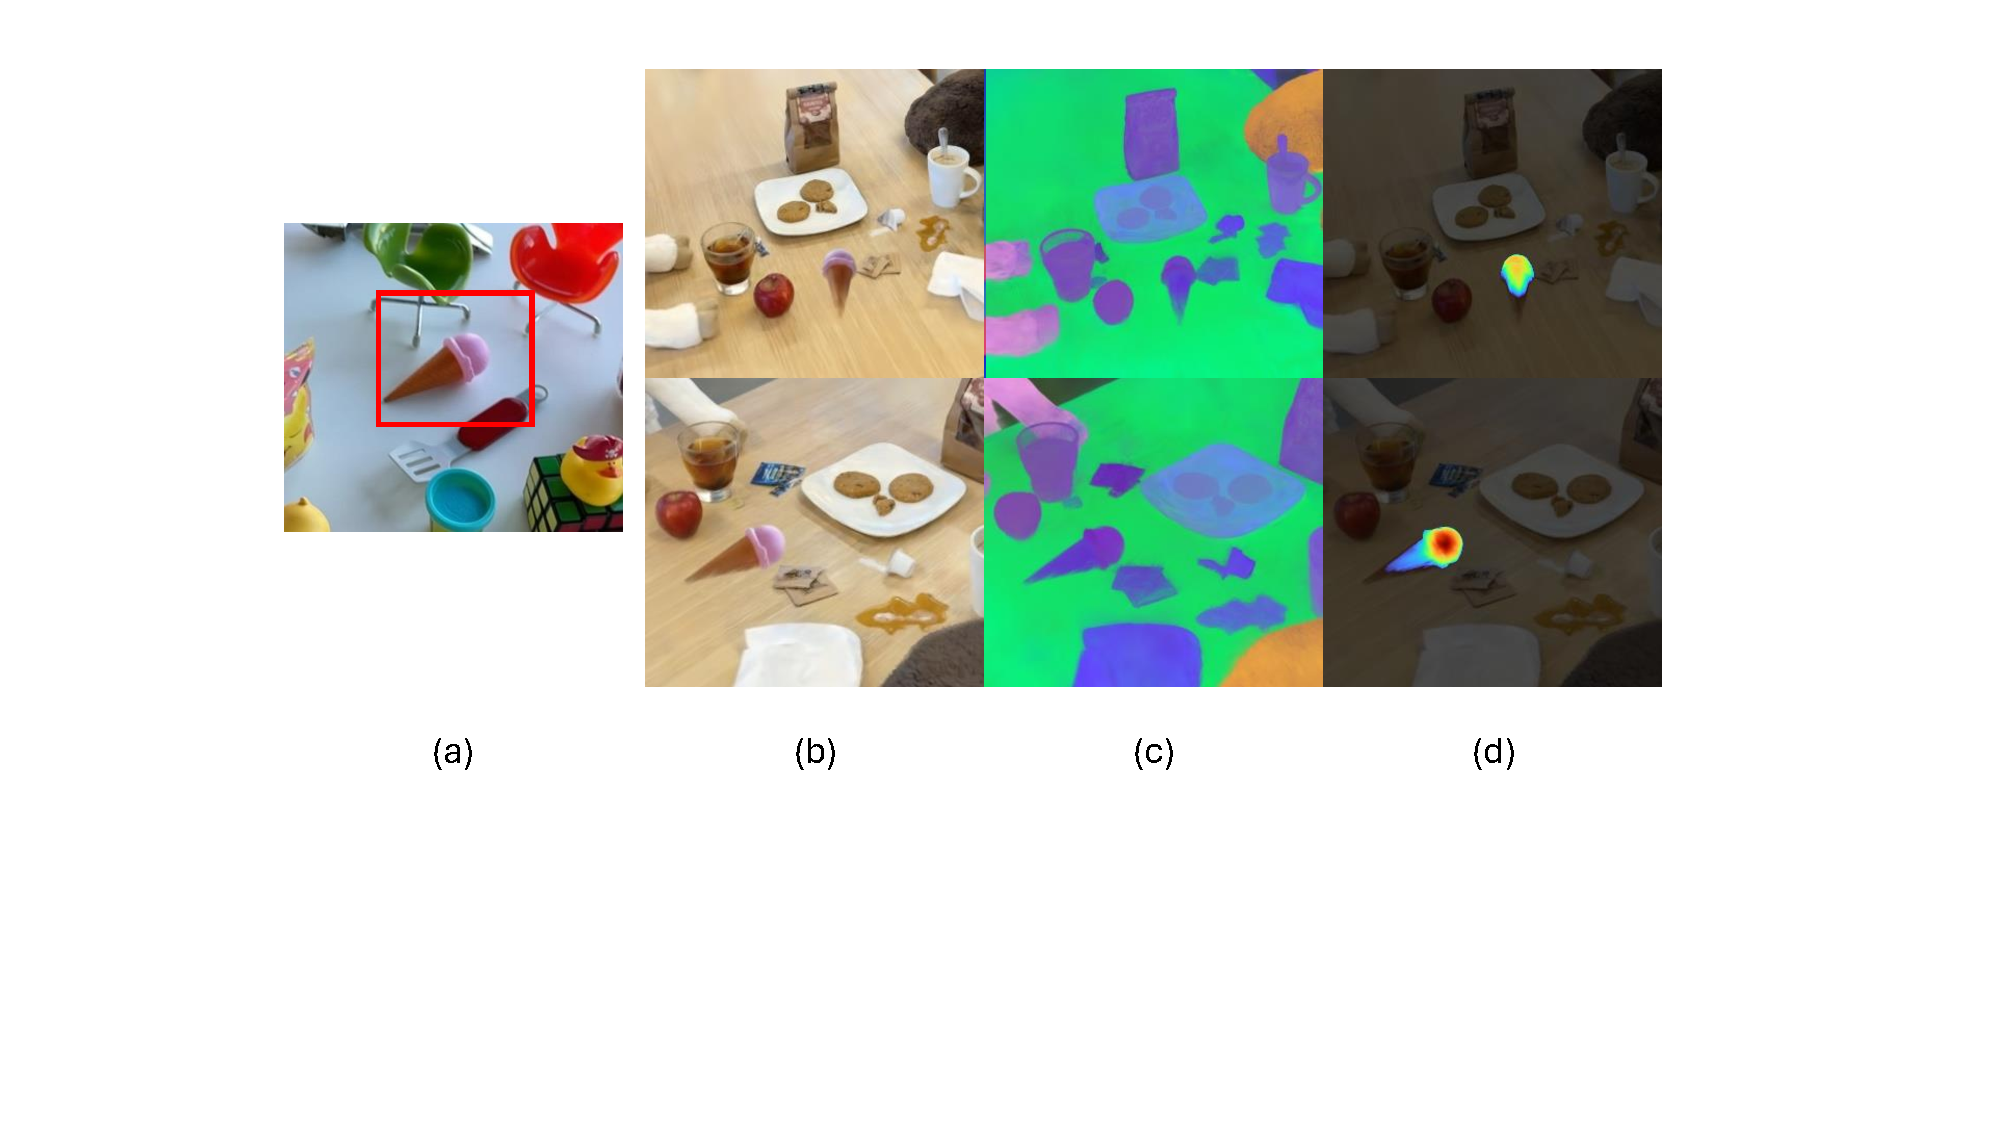
\includegraphics[trim={4.8cm 6cm 2cm 1cm}, clip, width=0.55\textwidth]{figures/obj_insertion.pdf}
    \caption{Visualization of Object Insertion: (a) Object Selection: An object is selected in the Figurines scene (b) Object Insertion: The object is transferred and integrated into the Teatime scene (c) Feature Analysis: PCA visualization of the feature map to show the object's integration in the semantic space (d) Query Visualization: Heatmap showing the response to the query ``pink icecream".}
    \label{fig:obj-insert}
\end{figure}

Our method's key advantage is integrating dense 3D language features into Gaussian Splatting with a simple representation. This allows us to profit from their strong open-set generalization capability and the advances in 2D language feature representations. This has the potential to enable a range of downstream 3D tasks, especially related to scene editing and interaction.

We demonstrate this capability on object insertion, where an object is taken from an existing 3D Gaussian Splat and integrated into another scene. While the current state-of-the-art LangSplat would require finetuning of the scene-specific language autoencoder, as well as the retraining of the whole feature embedding, our representation can be augmented with the new object similarly to any other Gaussian splat by simple copy-paste editing. As illustrated in Figure \ref{fig:obj-insert}, we select and extract an ice cream cone (represented by its Gaussians) from the Figurines scene of LERF~\cite{kerr2023lerf}. By simply copying the object's Gaussians together with their parameters and semantic features, the new object seamlessly integrates into the Teatime scene while preserving its semantic features. Then, we query the modified scene with "pink ice-cream". The resulting relevancy heatmap in Figure~\ref{fig:obj-insert})~(d) confirms that our method maintains the semantic understanding of the inserted object in its new context. This demonstrates that our approach enables direct semantic feature manipulation without scene-specific dimensional reduction, offering flexibility for practical editing while preserving semantic querying capabilities.
